\subsection{Glyph: \glyph{Compartment}}
\label{sec:compartment}

A compartment is a logical or physical structure that contains entity pool nodes. An EPN can only belong to one compartment. Therefore, the ``same'' biochemical entities located in two different compartments are in fact two different pools.

\begin{glyphDescription}

\glyphSboTerm  SBO:0000290 ! physical compartment

\glyphIncoming
None.

\glyphOutgoing
Zero or more \glyph{equivalence arcs} (\sect{equivalenceArc}).

\glyphContainer
A \glyph{compartment} is represented by a surface enclosed in a continuous border or located between continuous borders.
These borders should be noticeably thicker than the borders of the EPNs.
A compartment can take \textbf{any} shape.
A compartment must always be entirely enclosed.

\glyphLabel
A \glyph{compartment} is identified by a label that is  a string of characters that may be distributed on several lines to improve readability.
The label can be placed anywhere in the shape.
The label may extend outside of the shape.

\glyphAux
A \glyph{compartment} can carry one or more \glyph{units of information} (\sect{unitInfo}).
These can characterise the physical environment, such as pH, temperature or voltage.

\end{glyphDescription}

\begin{figure}[H]
  \centering
  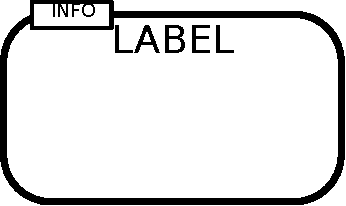
\includegraphics{images/build/compartment.pdf}
  \caption{The \PD glyph for \glyph{compartment}.}
  \label{fig:compartment}
\end{figure}

To allow more aesthetically pleasing and understandable maps, compartments are allowed to overlap each other visually, but it must be kept in mind that this does not mean the top compartment contains part of the bottom compartment.
\fig{overlap} shows two semantically equivalent placement of compartments:

\begin{figure}[H]
  \centering
  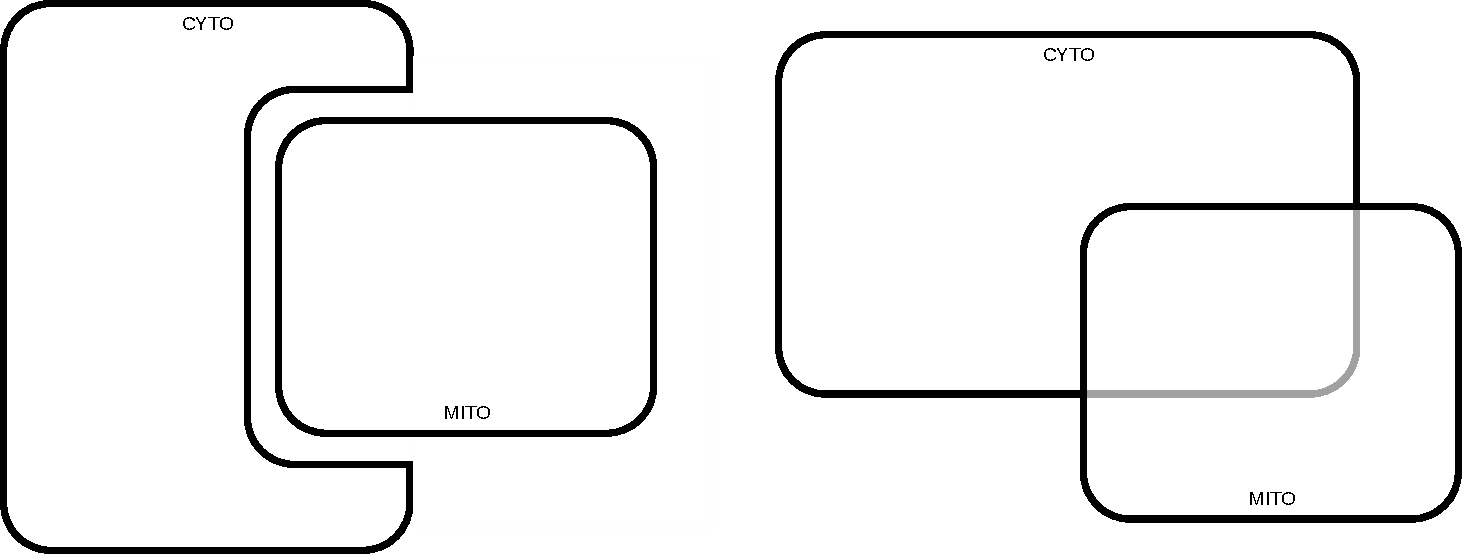
\includegraphics[scale = 0.5]{images/build/compartment_overlapping_example.pdf}
  \caption{Overlapped compartments are permitted, but the overlap does not imply containment.}
  \label{fig:overlap}
\end{figure}

